\chapter{ METHODOLOGY}

\noindent
In this chapter, we present the methodological framework adopted for our study (Figure \ref{fig:methodology_overview}). We detail the processes of data preparation, question-answer generation, model training, and evaluation. Each section outlines the specific steps and techniques employed to ensure the reproducibility of our results. For transparency, all prompts used in this research are included in the Appendix.

% TODO: specify that the dataset is question-code pairs

\begin{figure}[hbtp]
  \centering
  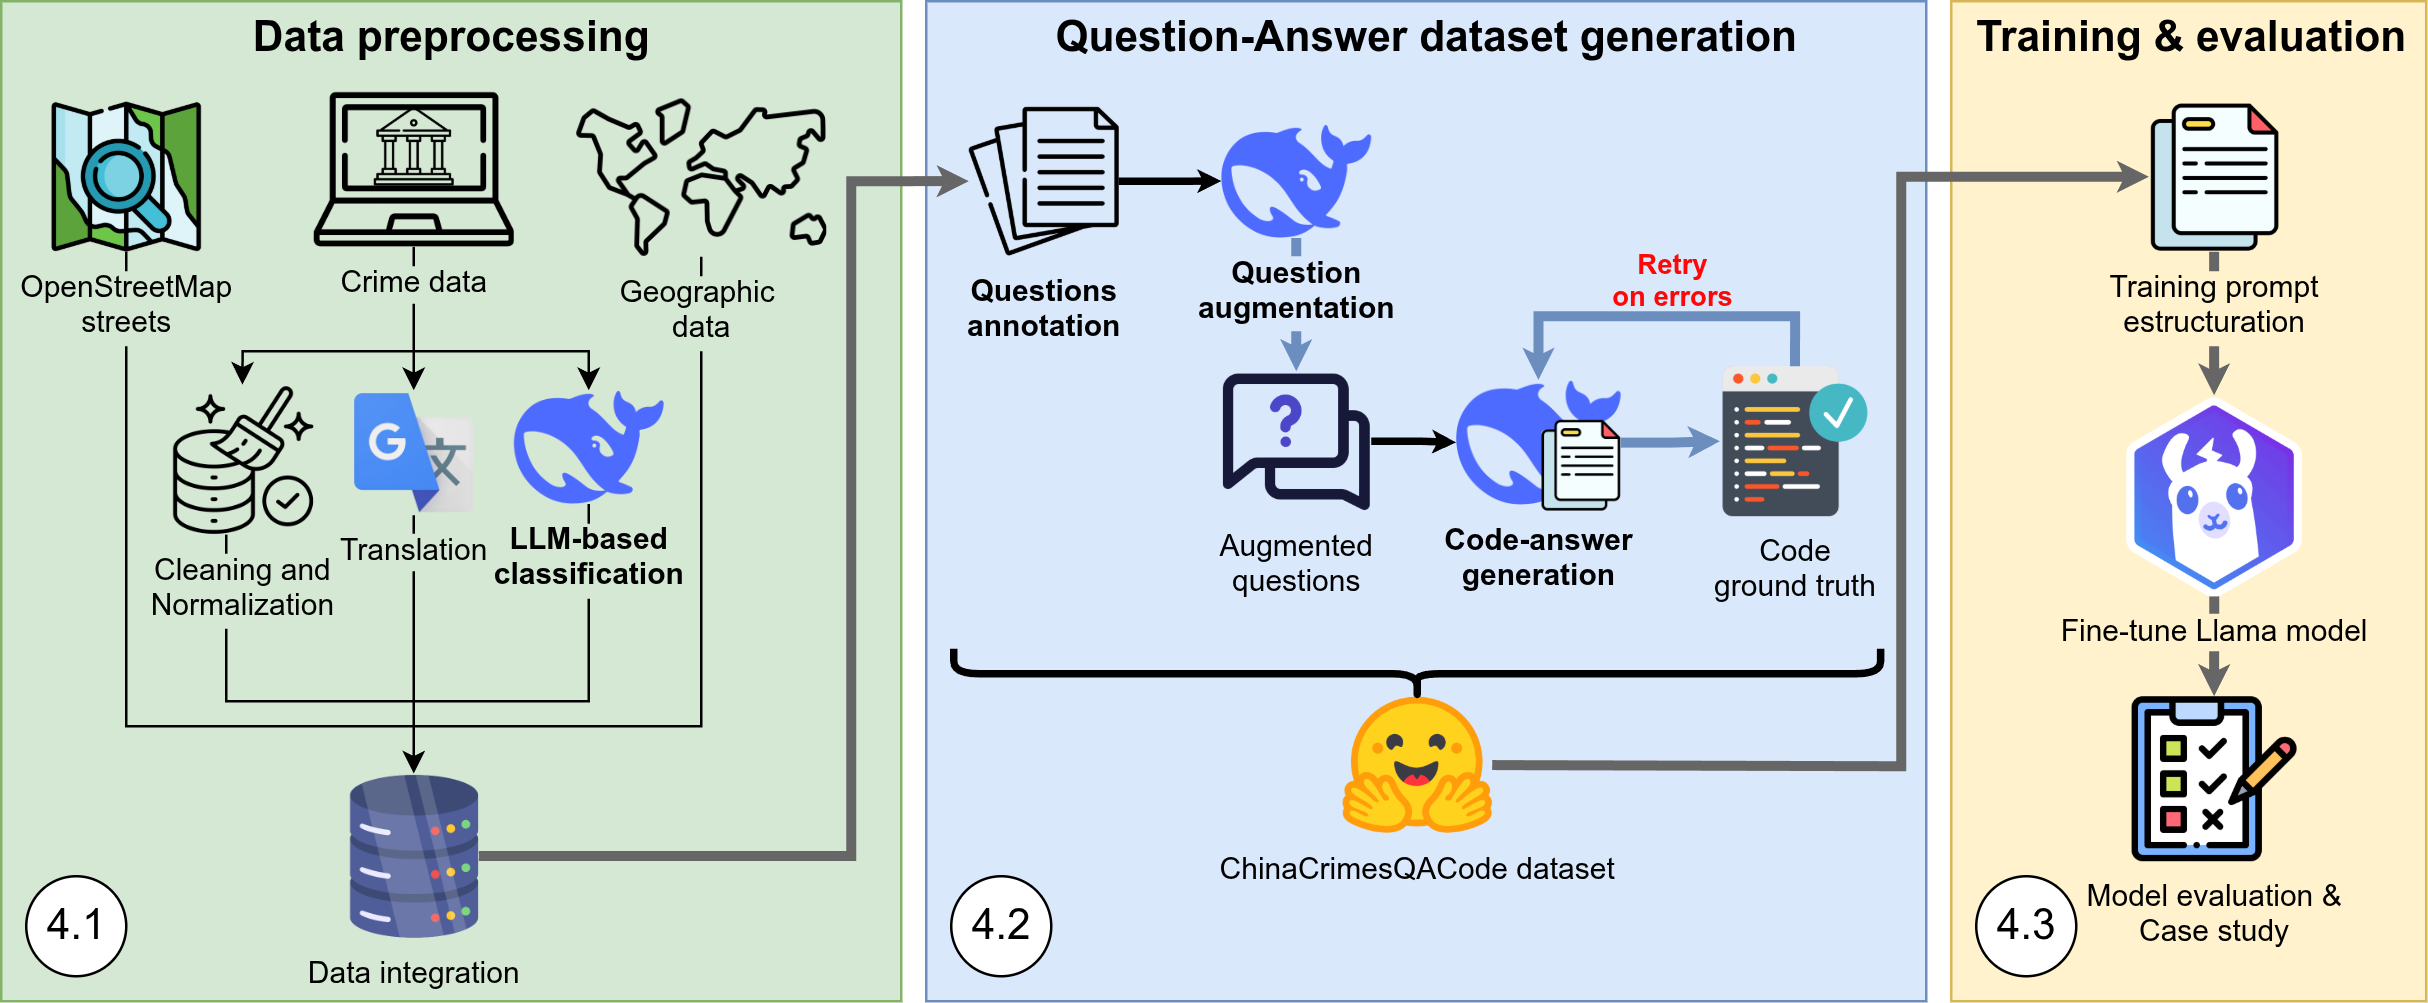
\includegraphics[width=\textwidth]{images/metodologiaExtended.png}
  \captionsetup{justification=raggedright,singlelinecheck=false}
  \caption{Methodology overview: First, we prepare the crime data by cleaning and normalizing the dataset, incorporating geographic boundaries and OpenStreetMap data. Next, we generate question-answer pairs using an open source LLM. Then, we fine-tune a Llama-3.1-8B model on these pairs. Finally, we evaluate the model's performance and implement an inference pipeline to conduct the case studies.}
  \label{fig:methodology_overview}
\end{figure}


\section{Data preprocessing}

\noindent
This section describes the procedures followed to curate and preprocess the datasets used in our research. We detail the selection of data sources, the integration of supplementary geographic and road network information, and the steps taken to ensure data quality and consistency prior to analysis.


\subsection{Data sources}

Our study utilizes the extensive China crime dataset published by \cite{Zhang2025CrimeDatasetChina}. We selected this dataset due to its substantial volume of data, extensive temporal coverage, and broad territorial scope. To provide geographic context, we incorporated administrative boundary data (containing polygon geometries for provinces, cities, and counties) from \cite{GeoJSON2025China} and complemented this with road network graph data from OpenStreetMap (\cite{Vargas2021OSM}). This integration enabled us to calculate spatial relationships between criminal incidents and transportation infrastructure, an important analytical dimension in our research. Comprehensive details of all dataset attributes are available in Appendix \ref{appendix:dataset}.

\subsection{Data sources cleaning and normalization}

The dataset underwent a comprehensive cleaning process to ensure consistency. First, we removed all rows with missing values in the \texttt{crimes\_df} dataframe, which contains the main crime data. Next, we translated all text fields to English using Google Translate, making the dataset accessible to a wider audience. We then standardized the date formats across all dataframes to ensure consistency in temporal analysis. After that, to reduce the number of categories in the \texttt{crime\_type} column, we applied a classification using a LLM (DeepSeekV3) to group similar crime types into broader categories. Finally, to maintain analytical focus, we filtered the dataset to retain only the three provinces with the highest crime incidence during the 2017–2019 period: \textit{Jiangsu}, \textit{Guangdong}, and \textit{Zhejiang}.

\section{Question-Answer dataset generation}

% TODO: improve introduction
% We develop a synthetic dataset named "ChinaCrimesQACode" that contains question-code pairs for crime data analysis. 
This section describes the methodology used to generate the question-answer pairs for our synthetic dataset. We detail how we designed the prompts to elicit accurate and functional code solutions from the DeepSeek V3 model, which serves as the backbone for generating answers to user queries.

\subsection{Question generation}

First, we created 100 question templates (inspired by \citep{Dai2024QASTKG, Contractor2020QATourism}), covering different types of inquiries including spatio-temporal, comparative, and causal questions about crime data. These templates were designed to be adaptable for crime datasets from other countries as well.

We expanded this initial set through question augmentation techniques used by \cite{Yin2024MuMathCode, Li2024MuggleMath, Jain2024MetaFineTuning}, specifically rephrasing (with temperature setting of 0.5) and alteration (with temperature setting of 0.75) via few-shot prompting (see prompts in Listings \ref{prompt:question_rephrasing} and \ref{prompt:question_augmentation})
. These question categories are summarized in Table~\ref{tab:question_types}. % see Table~\ref{tab:question_type_counts}, 

% \begin{table}[H]
% \centering
% \footnotesize
% \begin{tabular}{lr}
% \hline
% \textbf{Augmentation} & \textbf{\# count} \\
% \hline
% altered     & 3860 \\
% paraphrased & 1732 \\
% \hline
% \end{tabular}
% \caption{Distribution of question types in the dataset.}
% \label{tab:question_type_counts}
% \end{table}

\begin{table}[H]
\centering
\footnotesize
\begin{tabular}{ll}
  \toprule
\textbf{Question Type} & \textbf{Description} \\
\midrule
\texttt{spatial\_lookup} & Location-only questions \\
\texttt{temporal\_lookup} & Time-centric questions \\
\texttt{spatio\_temporal\_lookup} & Joint space-time filters \\
\texttt{comparative\_trends} & Rankings and evolution analysis \\
\texttt{causal\_contextual} & Event patterns and conditional queries \\
\texttt{hypotheticals\_counterfactuals} & Projections and counterfactual reasoning \\
\texttt{multi\_step\_aggregation} & Multi-step reasoning and aggregation \\
\bottomrule
\end{tabular}
\caption{Question types in the ChinaCrimesQACode dataset}
\label{tab:question_types}
\end{table}


\subsection{Code-answer generation}

For each original question type, we manually wrote one Python code solution to serve as a reference. These hand-crafted examples provided context for generating additional synthetic code answers using the DeepSeek V3 model, guided by a structured prompt and nucleus sampling \citep{Holtzman2020NucleusSampling, Ahmad2025OCRNVidia, Nvidia2024KaggleMath} with a top\_p value of 0.95. This allowed the model to explore diverse reasoning paths and alternative implementations.

The answer generation prompt (Figure~\ref{fig:answer_generation_prompt_structure}) follows a layered structure designed to guide the DeepSeek V3 model through a rich, contextualized reasoning process. At the top level, the \textbf{System Instructions} define the model’s role and restrict its scope of reasoning, ensuring consistency and relevance across generations. The \textbf{User Prompt} includes several critical components: the \textit{Dataset Context}, which introduces the \textit{Dataset Specification} of the three core dataframes (\texttt{crimes\_df}, \texttt{streets\_df}, and \texttt{geometries\_df}); one-shot \textit{Reference Material}, offering prior examples (reference question and code) to scaffold the model’s behavior; the target \textit{User Question}; and a \textit{Detailed Task Description} outlining specific rules, especially when the question is a rephrased or altered version of a known query.

Complementing this, the \textbf{Dataset Specification} explicitly lists the column names, sample rows, data types, and semantic descriptions of each field, encouraging schema awareness and reducing ambiguity during code generation. An \textbf{Output Format} section further prescribes the XML response schema to enforce structured and machine-readable outputs.

With this prompt (adaptable to both paraphrased and altered questions), we executed code generation attempts in a loop, verifying each output through assertions, code execution, and consistency checks. If the output failed, we resubmitted the query to the LLM until a valid solution was obtained or the maximum retry limit (set to 3) was reached. Additionally, for paraphrased questions, we used functional equivalence prompts to ensure that newly generated solutions and answers were aligned with the reference implementation.

\begin{figure}[H]
  \centering
  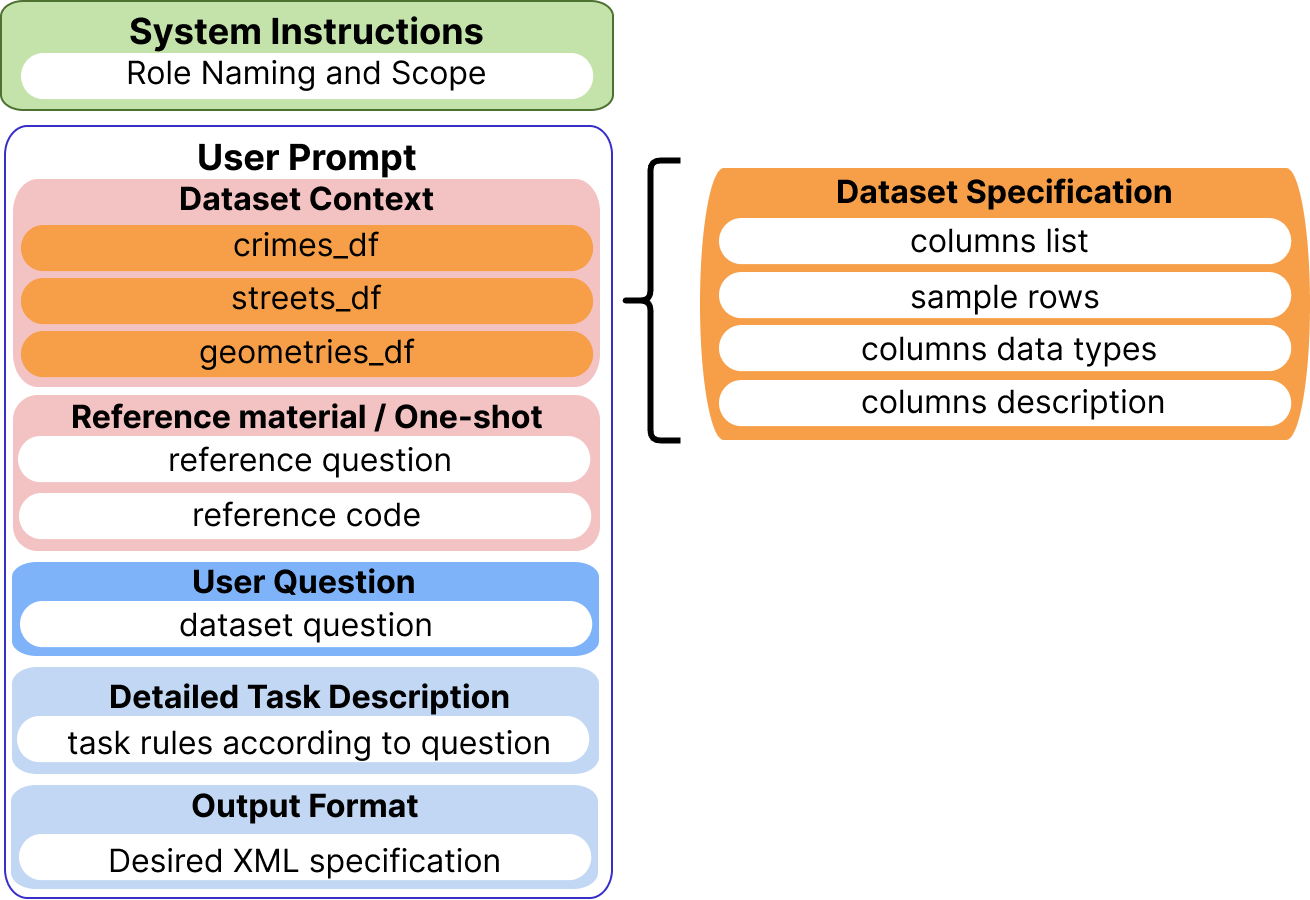
\includegraphics[width=0.65\textwidth]{images/answer_gen.png}
  \caption{Answer generation prompt structure}
  \label{fig:answer_generation_prompt_structure}
\end{figure}


\subsection{Dataset curation and splitting}

To ensure quality, we verified that all LLM-generated Python solutions executed correctly. After that, we dropped the questions with no valid code solutions (limit exceeded, code with errors, or no code generated). Finally, we conducted manual reviews of all question-answer pairs to guarantee their quality.

The resulting dataset, which we named "ChinaCrimesQACode", contains around 5,000 question-code solution pairs, representing an adequate sample volume for effective model training \citep{Unsloth2024Dataset1}. We divided the dataset into training and test subsets using an 80/20 split to facilitate robust model training and comprehensive evaluation. The dataset is publicly available on HuggingFace for further research and development.  %  (Table~\ref{tab:dataset_split})
% This review process involved verifying that the answers were accurate, relevant, and aligned with the corresponding questions. We also ensured that the answers were concise and clear, making them suitable for use in our visualization tool.

% \begin{table}[H]
% \centering
% \begin{tabular}{lr}
% \hline
% \textbf{Split} & \textbf{Count} \\
% \hline
% train & 4513 \\
% test  & 1079 \\
% \hline
% \end{tabular}
% \caption{Dataset split distribution.}
% \label{tab:dataset_split}
% \end{table}


% TODO: poner ejemplo de question-answer pair

% \section{Dataset generation}

% This section describes the methodology used to generate the question-answer pairs for our dataset, focusing on the structured prompts and the code generation process. We detail how we designed the prompts to elicit accurate and functional code solutions from the DeepSeek V3 model, which serves as the backbone for generating answers to user queries.

% \subsection{Prompt Structuration}

% All prompts were carefully designed to ensure the model understood the task requirements and could generate accurate code solutions. We describe below the structure of the prompts used both for answer generation and model training, highlighting how each layer of context helps to elicit precise and functional responses from the model. Full prompt examples are included in Appendix~\ref{appendix:prompts} for transparency and reproducibility.


\section{Training and evaluation}

This section outlines the process of training and evaluating our fine-tuned Llama-3.1-8B model, covering prompt design, model selection, training setup and assessment metrics used.


\subsection{Training prompt structure}

The training prompt (Figure~\ref{fig:training_prompt_structure}) was designed to fine-tune the model toward robust code generation. It follows a layered structure similar in philosophy to the answer generation prompt (Figure~\ref{fig:answer_generation_prompt_structure}), but introduces stricter constraints and excludes example-based reasoning to encourage generalization. Specifically, the training prompt follows a zero-shot setup—forcing the model to synthesize reasoning paths from schema knowledge and natural language instructions alone, without relying on reference code.

At the top level, the \textbf{System Instructions} define the model’s identity as a geospatial crime analytics expert and restrict the environment to specific, pre-approved libraries. This promotes deterministic and reproducible outputs by reducing spurious library imports and implementation drift.

The \textbf{User Prompt} includes three main elements. First, the \textit{Dataset Context} outlines the structure and semantics of the three core GeoDataFrames, \texttt{crimes\_df}, \texttt{streets\_df}, and \texttt{geometries\_df}, and highlights their interrelations (e.g., spatial joins, containment logic). Second, the \textit{User Question} presents the target query in plain language. Finally, the \textit{Critical Requirements} specify functional and implementation-level constraints, such as required function signatures, alignment of coordinate reference systems (CRS), and the use of robust error handling.

Unlike the answer generation prompt, no reference examples or prior code are provided. This intentional omission reinforces the model's ability to infer behavior solely from structural schema understanding and task requirements.

Lastly, an explicit \textbf{Output Format} section mandates that the model must produce a single Python code block with no additional explanations or comments. This ensures compatibility with downstream evaluators and enables automatic execution. An \textbf{Execution Directive} enforces this behavior from the first token, guaranteeing a clean, code-first output.

\begin{figure}[H]
  \centering
  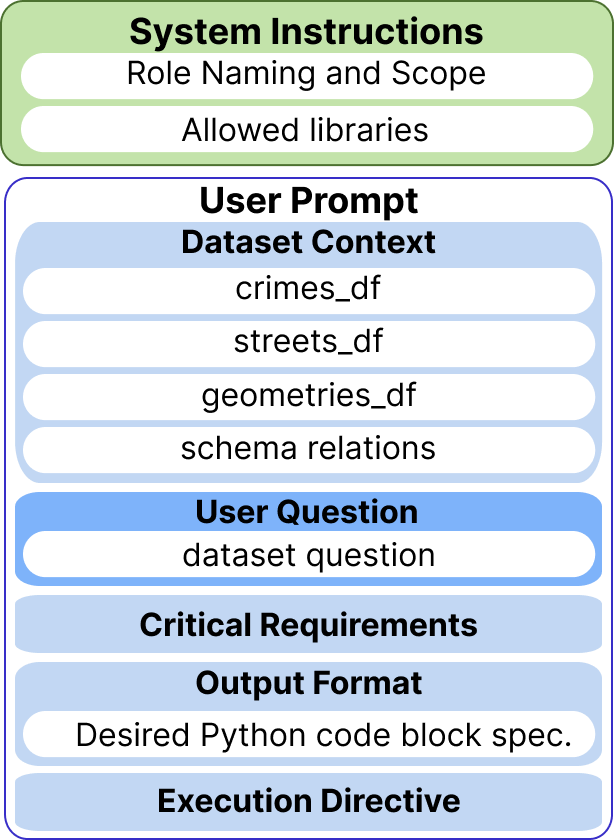
\includegraphics[width=0.3\textwidth]{images/prompt.png}
  \captionsetup{justification=raggedright,singlelinecheck=false}
  \caption{Training prompt structure: Divided into two main sections. The first section outlines the system instructions, specifying the model's role and permitted libraries. The second section contains the user prompt, which includes the dataset context, user question, and critical requirements.}
  \label{fig:training_prompt_structure}
\end{figure}


\subsection{Model Fine-Tuning}

We fine-tuned the Llama-3.1-8B Instruct model \citep{Grattafiori2024Llama3, Unsloth2024WhatModel} by implementing the techniques described in \cite{Pareja2024RecipesSFT}. For the fine-tuning process, we utilized Hugging Face Transformers alongside the Unsloth library to optimize computational resources and accelerate training, completing the entire procedure in approximately 3 hours using a single NVIDIA H100 GPU with 80GB memory provided by Lightning AI. This model was chosen as it represents a balance between size (8B), data science coding capabilities \citep{Lai2022DS1000}, and compatibility with Unsloth for fast and efficient fine-tuning.



\subsection{Model Evaluation}

% We adopted the approach proposed by \citep{Fleureau2024NuminaMath}, Self-Consistency Tool-Integrated Reasoning (SC-TIR) to evaluate our fine tuned model
For model evaluation, we adopted a comprehensive approach combining both automated and LLM-based assessment methods. Specifically, we used pass@k \citep{Levi2024SimpleModelInferenceScalingLaws} (with $k=16$ and multinomial sampling), where correctness was determined using an LLM-as-a-judge \citep{Li2025LLMJudge} (Appendix~\ref{appendix:prompts}) using GPT-4.1, and CodeBLEU \citep{Ren2020CodeBLEU}, which provides a purely quantitative measure of code generation quality. Additionally, we calculated the error percentage across all generated code samples to assess overall robustness. Finally, we performed Tool Integrated Reasoning (TIR) \citep{Fleureau2024NuminaMath} evaluations, allowing a single retry per question to mitigate frequent inference errors such as ZeroDivisionError and IndexError, while maintaining evaluation efficiency.

% TODO: poner que metodo de inferencia estamos usando, puede que sea greedy decoding

% The model was trained using QLoRA \citep{Dettmers2023QLoRA} with a rank of 64, alpha of 16, and a dropout rate of 0.05. 

% We employed a learning rate of 2e-4 with the AdamW optimizer and cosine learning rate scheduler with 100 warm-up steps. Training was performed for 3 epochs with a batch size of 16, using a maximum sequence length of 2048 tokens. To maintain training stability, we applied gradient clipping with a maximum norm of 1.0.

% For instruction tuning, we formatted our question-code pairs using a standard template that clearly specified the task context and expectations. Each question was prefaced with a system prompt indicating that the model should generate executable Python code to analyze crime data and answer the given question. 


\section{Inference Workflow}

This section describes the inference pipeline implemented for our case studies, detailing the process from user query to final response. As illustrated in Figure~\ref{fig:inference_pipeline}, the workflow consists of several key stages: first, the user query is processed by a fine-tuned Llama3-8B model, which generates multiple code solutions. Each code snippet is executed to produce corresponding outputs. Finally, a Llama3-8B-Base model performs summarization of these results to create the final response presented to the user.
%  This architecture enables robust and accurate responses to complex geospatial crime analytics queries.

\begin{figure}[H]
  \centering
  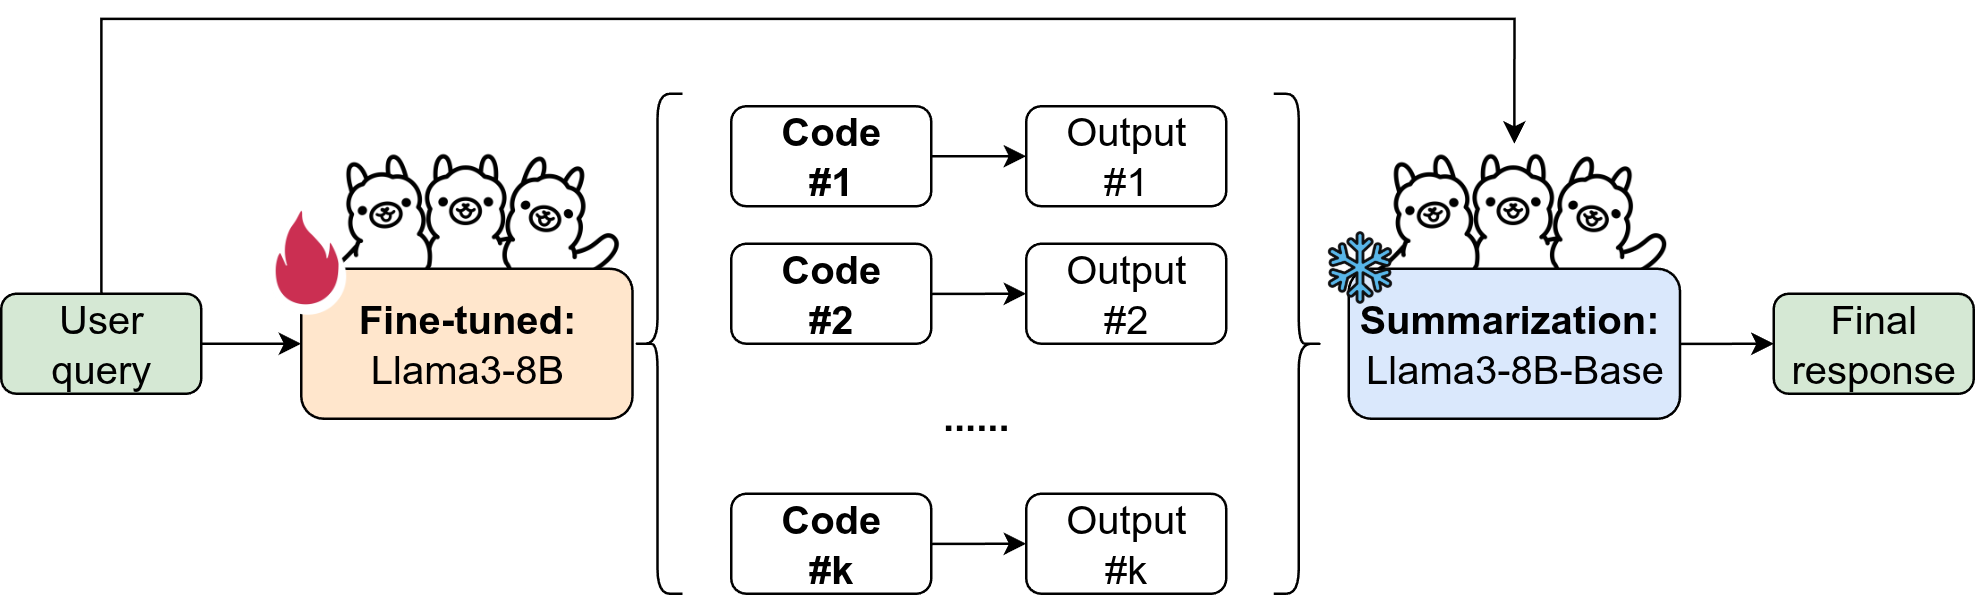
\includegraphics[width=0.9\textwidth]{images/inference_pipeline.drawio.png}
  \caption{Chat inference pipeline}
  \label{fig:inference_pipeline}
\end{figure}

\section{Summary}

This methodology chapter presented a comprehensive framework for crime data analysis through natural language queries. Beginning with dataset preparation using Chinese crime data, administrative boundaries, and road networks, we detailed the data cleaning process and focused on three high-crime provinces. We then described our question-answer dataset creation through template-based generation, augmentation techniques, and code generation using DeepSeek V3. Our prompt engineering utilized structured contexts for both answer generation and model training. We fine-tuned the Llama-3.1-8B model using Unsloth for computational efficiency, and employed multiple evaluation metrics including pass@k and CodeBLEU. Finally, we outlined our inference workflow that leverages multiple code solutions to provide accurate responses to user queries about crime analytics.
